\chapter{Sviluppo}
\label{chap:development}

\textit{In questo capitolo viene trattato il processo di sviluppo, le funzionalità sviluppate, il lavoro svolto, i problemi incontrati, le soluzioni adottate e i prodotti finali ottenuti}

\section{Assistente backend Jira}

\subsection{Introduzione}
L'obiettivo è la realizzazione di un assistente AI che possa semplificare il lavoro di un operatore umano durante l'attività di supporto tecnico generando una proposta di risoluzione ai biglietti di supporto aperti su Jira. Il LLM riceverà attraverso la tecnica della \textit{Retrieval Augmented Generation} biglietti risolti in passato che trattavano un problema simile sulla stessa componente. Una volta risolto, tale biglietto verrà a sua volta archiviato con la risoluzione del problema in modo da poter essere utilizzato in futuro.  

\subsection{Sprint 1 - Studio tecnologie}
Il primo Sprint è stato dedicato totalmente allo studio della documentazione fornita dai tutor sulle principali tecnologie che sarebbero state utilizzate durante lo stage o conoscenze ritenute necessarie per comprendere il codice esistente e il suo funzionamento, sviluppato dal compagno di progetto.
Ho perciò consultato il materiale fornito riguardante:
\begin{itemize}
    \item sviluppo Agile e \textit{framework} Scrum;
    \item Node.js, Node Version Manager(NVM), Javascript e Typescript;
    \item i Servizi Web di Amazon, in particolare Bedrock e Lambda;
    \item MongoDB come data e \textit{vector store};
    \item GitHub e Git.
\end{itemize}

\subsubsection*{Ricerca Vettoriale}
Ho studiato con maggiore attenzione il funzionamento della \textbf{Ricerca Vettoriale} e come questa è stata implementata all'interno di MongoDB con la funzionalità di \textit{Atlas Search}:
all'interno della base di dati è necessario configurare un indice di ricerca apposito dove vanno specificati \textbf{path} (il nome del campo contenente l'\textit{embedding}), \textbf{numDimensions} (la dimensione del vettore numerico), \textbf{similarity} (similarità semantica calcolata) e \textbf{type} (tipologia di indice). \\
L'indice utilizzato nel progetto per il recupero dei biglietti con modelli locali è mostrato nel codice \ref{listing:vector_index_tickets_local}.

\begin{listing}[H]
    \begin{minted}[bgcolor=lightgray]{js}
    {
        "fields": [
            {
                "path": "embedding_local",
                "numDimensions": 768,
                "similarity": "cosine",
                "type": "vector"
            }
        ]
    }
    \end{minted}
    \caption{Indice vettoriale per ticket con modelli locali}
    \label{listing:vector_index_tickets_local}
\end{listing}

Nel database sono stati configurati due indici vettoriali in quanto, come verrà spiegato in seguito qui \ref{sec:choosing_local_models}, l'assistente utilizza sia i modelli Bedrock che quelli locali in sequenza per generare la proposta di risoluzione e per il salvataggio nel database.

\subsubsection*{Implementazione della RAG}

In seguito mi sono dedicato ad approfondire la tecnica della \textbf{Retrieval Augmented Generation} e consultare guide su come implementarla. 
In particolare, la seguente\footcite{site:rag-impl-guide} è stata particolarmente utile e comprensiva: viene illustrato passo per passo come realizzare un chatbot che utilizzi la RAG, completamente in locale,
implementata con Ollama per l'esecuzione di LLM, Chroma come \textit{vector store}, LangChain in quanto una delle migliori librerie quando si tratta di realizzare un'applicazione nel campo AI grazie alle sue molteplici integrazioni disponibili e Streamlit per costruire l'interfaccia del chatbot velocemente.\\

\subsubsection*{Llama.cpp vs Ollama}
Infine ho studiato le soluzioni disponibili per l'esecuzione di LLM localmente, confrontando \textbf{Llama.cpp} e \textbf{Ollama}. 
Entrambi permettono di installare ed eseguire modelli localmente su hardware di uso comune senza la necessità di schede video di fascia alta o specializzate, sfruttando la quantizzazione, tecnica di compressione dei modelli dove diminuendo la precisione nella rappresentazione numerica in bit dei pesi, 
si riduce la loro dimensione e l'occupazione di memoria al costo di peggiorare leggermente le prestazioni. \\
Per il progetto ho optato per Ollama, abbreviazione di "Optimized LLaMA", realizzato proprio a partire da Llama.cpp, ma presentando varie migliorie:
\begin{itemize}
    \item \textbf{più semplice da installare ed impostare} l'ambiente locale;
    \item \textbf{facilità di utilizzo} in quanto gestisce automaticamente la formattazione delle richieste di chat nel formato previsto da ciascun modello e carica e scarica i LLM su richiesta in base a quello richiesto da una \textit{client Application Programming Interface(API)};
    \item possibilità di \textbf{personalizzare i modelli} disponibili in libreria attraverso il \textit{Modelfile} con cui si può modificare parametri, ad esempio il messaggio di sistema, la temperatura e la dimensione della \textit{context window};
    \item \textbf{ampia libreria} contenente i migliori LLM \textit{Open Weight} disponibili, con la possibilità di importarne altri convertendoli nel formato \textit{GPT Generated Unified Format}.
\end{itemize}

\subsection{Sprint 2 - Sviluppo modulo LLM locale sostitutivo}
Durante il secondo \textit{Sprint} in parallelo allo studio delle tecnologie, ho cominciato a svolgere attività più pratiche, iniziando scrivendo piccoli script e aiutando nella stesura delle domande di benchmark, fino a sviluppare grossa parte del modulo AI alternativo con modelli locali. 

\subsubsection*{Studio tecnologie e codice esistente}
Per poter iniziare a lavorare efficientemente con i modelli localmente, prima di tutto ho 
impostato l'ambiente locale sul mio computer fisso affinché potessi eseguire i modelli AI scaricati da Ollama sfruttando l'accelerazione hardware della scheda video NVIDIA a mia disposizione. 
A tal fine ho installato l'immagine dello strumento, disponibile su Docker Hub, sul sottosistema Windows per Linux (WSL) in quanto è l'unico modo in cui Docker Desktop supporta l'utilizzo della GPU.
I passaggi fatti sono stati:
\begin{enumerate}
    \item scaricare e configurare NVIDIA Container Toolkit e NVIDIA Cuda per WSL;
    \item scaricare l'immagine di Ollama su WSL con l'opzione di utilizzo della scheda video;
    \item avviare Ollama e scaricare i modelli che si vogliono utilizzare.
\end{enumerate}
Inoltre ho sviluppato uno script per approfondire le mie competenze e fare pratica con le tecnologie, sfruttando le integrazioni offerte dal \textit{framework} LangChain per connettermi a un database MongoDB.
Lo script consente di aggiungere e recuperare documenti dal database e di fornire questi a un modello AI eseguito su Ollama.\\
Infine ho iniziato lo studio del codice esistente.

\subsubsection*{Benchmark e scelta modelli locali}
\label{sec:choosing_local_models}

Con l'ambiente di lavoro impostato e pronto, era ora di individuare i modelli AI che avrei utilizzato localmente.\\

Per la scelta del LLM locale che avrebbe generato le proposte di risoluzione, ho 
utilizzato il \textit{benchmark} progettato dal compagno di stage: a ciascun modello vengono forniti 30 ticket di test con una varietà di contenuti e complessità al fine di determinare se le proposte di soluzione generate per ciascun biglietto fossero simili a quelle che si aspettava. 
Questa similarità veniva determinata dal modello \textit{cloud} \textbf{Mistral Large}, il migliore tra quelli offerti da AWS Bedrock, il quale forniva un punteggio variabile tra 0 (risposta totalmente diversa) a 1 (risposta identica). Infine, per ciascun modello veniva determinato il numero complessivo di domande a cui ha risposto in modo accettabile in base a tre soglie di punteggio: \textit{Low} (> 0.57), \textit{Medium} (> 0.65) e \textit{Strict} (> 0.72).

\begin{figure}[H]
    \centering
    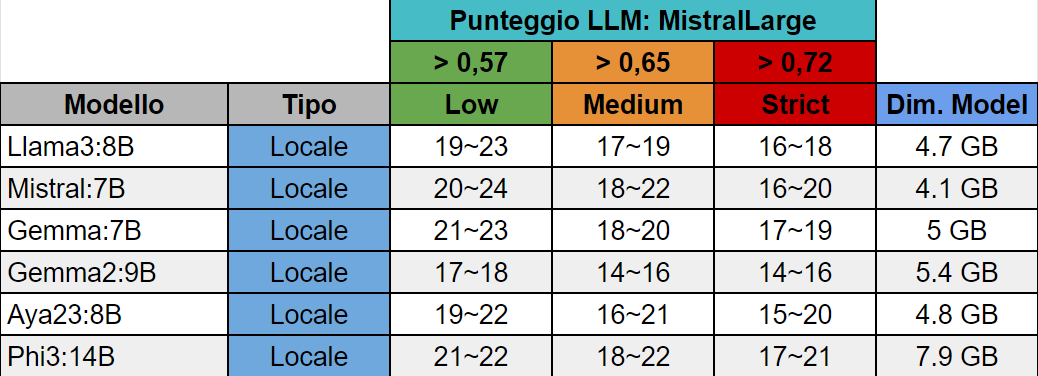
\includegraphics[alt={Tabella con risultati del benchmark sui LLM locali}, width=1\columnwidth]{img/benchmarkLLMlocali.png}
    \caption{Risultato del benchmark svolto sui LLMs locali}
    \label{fig:results_local_llms}
\end{figure}

I risultati del test, rappresentati in Figura \ref{fig:results_local_llms}, hanno mostrato che in media il modello \textbf{Mistral 8B} ha risposto in modo accettabile al maggior numero di risposte per ciascuna soglia di punteggio. 

\textcolor{notaBeneBlue}{\textbf{Nota Bene}: Il benchmark era utile per individuare 
modelli in grado di proporre le risposte correttamente,ma era anche molto restrittivo sul 
formato della risposta: dovevano essere formulate come un’unica frase che contenesse anche
multiple soluzioni. Tuttavia dato che il prompt utilizzato per i modelli era molto 
generico, modelli come Gemma2 e Aya che producevano la risposta con un formato differente, 
ad esempio frasi singole per ogni proposta di risoluzione, hanno ricevuto un punteggio 
complessivo basso, nonostante la risoluzione generata fosse corretta. 
Quindi modificando i prompt, inserendo istruzioni più precise e specifiche per ogni modello probabilmente avrebbe migliorato lo score di alcuni di essi.\\}

Al fine di mantenere il modulo LLMs locali completamente separato e indipendente da quello AWS Bedrock, si è 
deciso di utilizzare anche un modello di Embedding differente in locale per la generazione del vettore numerico sia per la 
ricerca vettoriale di argomenti simili da fornire al LLM locale che per il salvataggio dei ticket risolti nel database. 
Ho selezionato i modelli da testare consultando la classifica Massive Text Embedding Benchmark (MTEB) su HuggingFace, tenendo conto allo stesso tempo se fossero già presenti nella libreria di Ollama.\\
Il test consisteva nello svolgere la ricerca vettoriale di un ticket riguardante un problema con un microfono all’interno di un database di prova nel quale vi erano 3 documenti che trattavano la stessa problematica e la stessa componente.
I modelli di Embedding hanno generato il vettore numerico sia per il nuovo ticket che per quelli già salvati. 
Per ognuno venivano recuperati i 10 biglietti più simili attraverso la Ricerca Vettoriale ed è stato controllato:
\begin{itemize}
    \item se i 3 ticket più simili riguardassero la stessa problematica per la stessa componente;
    \item se ci fosse un distacco significativo tra lo score di similarità dei 3 ticket simili e i rimanenti 7.
\end{itemize}
In caso di parità dei risultati, viene scelto il modello più piccolo. 

\begin{figure}[H]
    \centering
    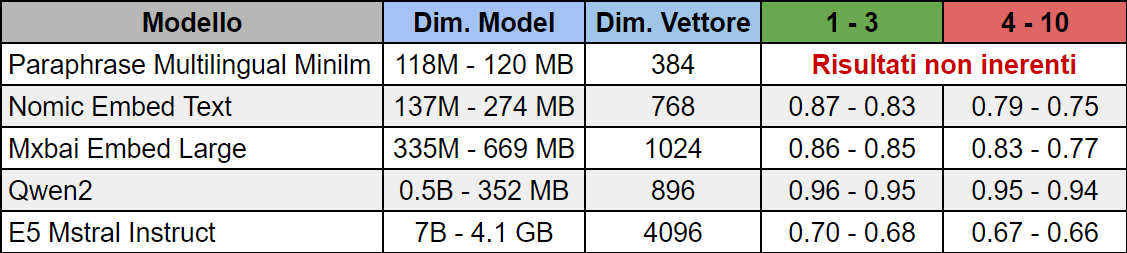
\includegraphics[alt={Tabella con risultati del benchmark sui modelli di Embedding locali}, width=1\columnwidth]{img/EmbeddingModelsLocal.png}
    \caption{Risultato del benchmark svolto sui modelli di Embedding locali}
    \label{fig:results_local_emb_models}
\end{figure}

In base ai risultati ottenuti, osservabili nella Figura \ref{fig:results_local_emb_models}, il modello selezionato è stato
il \textbf{Nomic Embed Text}, modello specializzato sul task di creazione di \textit{embedding} con solo 137 Milioni di parametri.

\newpage
\subsubsection*{Sviluppo modulo LLM locali}

Il funzionamento dell'assistente è incentrato su due funzioni di AWS Lambda.

\begin{figure}[H]
    \centering
    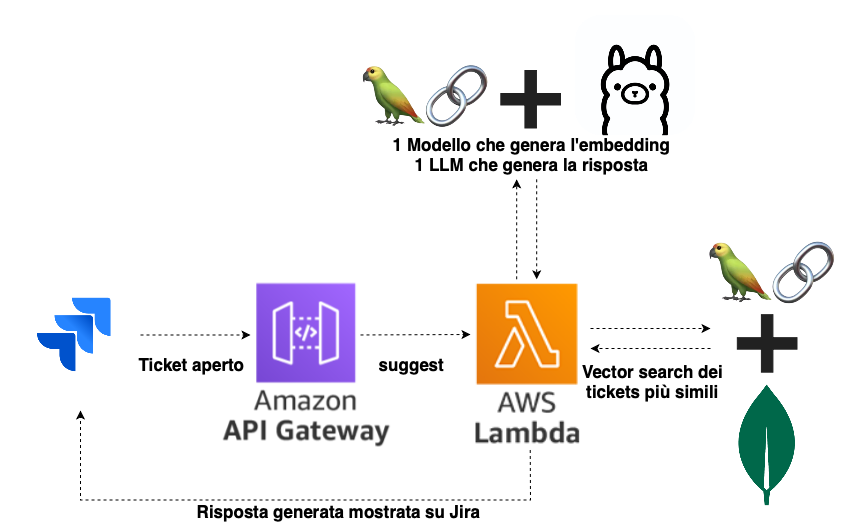
\includegraphics[alt={Flusso di esecuzione per la generazione di una risposta}, width=1\columnwidth]{img/ticketCreatoLocale.png}
    \caption{Flusso di esecuzione per un ticket aperto usando LLM locali}
    \label{fig:flow_chart_new_ticket}
\end{figure}

Il flusso di esecuzione per la generazione di un risposta, mostrato in Figura \ref{fig:flow_chart_new_ticket}, parte dalla Lambda \textbf{suggest}, la quale viene attivata quando su Jira viene creato un nuovo ticket di supporto.
\begin{enumerate}
    \item La funzione riceve il nuovo biglietto ed estrae il contenuto dei campi \textbf{summary} (titolo), \textbf{description} (descrizione del problema) e \textbf{components} (codice della componente) per creare una stringa unica; 
    \item questa verrà fornita al modello locale Nomic Embed Text per generare il vettore di \textit{embedding}, utilizzato per interrogare il database MongoDB tramite ricerca vettoriale per recuperare i 3 ticket risolti più simili;
    \item i documenti vengono restituiti alla funzione Lambda, la quale procede nuovamente ad estrarre il contenuto dei 3 campi sopra citati più \textbf{resolution description} (soluzione che ha funzionato);
    \item viene chiamato il modello Mistral 8B per la generazione della proposta di risoluzione: ciascun modello presenta un prompt personalizzato contenente informazioni di contesto, comandi su come generare la proposta di risoluzione e le informazioni recuperate dal database per aiutare il modello a rispondere in modo accurato;
    \item infine, il suggerimento su come risolvere il problema viene infine rimandato a Jira e stampato nel campo dedicato \textbf{Proposta di risoluzione}.
\end{enumerate}

\begin{figure}[H]
    \centering
    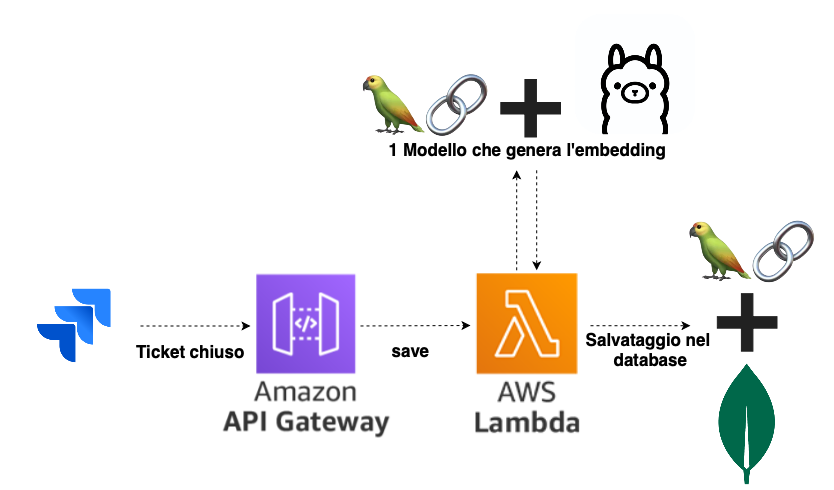
\includegraphics[alt={Flusso di esecuzione il salvataggio di un ticket chiuso}, width=1\columnwidth]{img/ticketChiusoLocale.png}
    \caption{Flusso di esecuzione per un ticket chiuso usando LLM locali}
    \label{fig:flow_chart_closed_ticket}
\end{figure}

La seconda Lambda \textbf{save} viene invocata alla chiusura di un ticket di supporto, come si può vedere dalla Figura \ref{fig:flow_chart_closed_ticket}.
\begin{enumerate}
    \item La funzione riceve il ticket che è stato chiuso ed estrae il contenuto dei campi \textbf{summary} (titolo), \textbf{description} (descrizione del problema), \textbf{components} (codice della componente) e \textbf{resolution description} (soluzione che ha funzionato) per creare una stringa unica; 
    \item questa verrà fornita al modello locale Nomic Embed Text per generare il vettore di \textit{embedding} che verrà salvato assieme al ticket, nel campo apposito \textbf{embedding local};
    \item infine il biglietto viene salvato all'interno del database MongoDB per l'uso in futuro.
\end{enumerate}

\subsection{Sprint 3 - Ultime migliorie}

Durante questo sprint ho ultimato il modulo con LLMs locali:
\begin{itemize}
    \item sono state fatte delle aggiunte al prompt del modello in modo che nella risposta generata vengano forniti anche dei link funzionanti ai ticket simili che sono stati recuperati attraverso la Ricerca Vettoriale e utilizzati durante la generazione, oltre a fornire un esempio di risposta attesa;
    \item terminato l'integrazione del modulo con modelli locali con il sistema esistente in modo che venga avviata la generazione della proposta di soluzione una volta aperto un ticket di supporto e venga poi stampata su Jira appena sia finito tale processo;
    \item aggiunti dei messaggi che vengono visualizzati durante la generazione per fornire un feedback visivo all'utente che tale processo è in corso;
    \item attività di testing finale per individuare eventuali bug o rifiniture da applicare.
\end{itemize}

\newpage
\subsection{Prodotto finale}

Il \textit{Proof of Concept} sviluppato dell'assistente, per richiesta del tutor, svolge entrambe le funzionalità di generazione della proposta di risoluzione e dell'archiviazione dei ticket di supporto risolti utilizzando prima i modelli \textit{cloud} di AWS Bedrock e poi quelli locali eseguiti su Ollama.
Infatti, come si può vedere in Figura \ref{fig:responses_example}, per ciascun biglietto di supporto tecnico, l'assistente AI genererà due proposte di risoluzione, stampate nei rispettivi campi testuali.

\begin{figure}[H]
    \centering
    
\includegraphics[alt={Esempio di ticket di supporto con le due proposte di risoluzione generate}, width=1\columnwidth]{img/responseGenerated.png}
    \caption{Esempio di ticket di supporto con le due proposte di risoluzione generate}
    \label{fig:responses_example}
\end{figure}

L'architettura complessiva del sistema locale, rappresentata nella Figura \ref{fig:jira_ai_architecture}, è composta da 4 componenti principali:
\begin{enumerate}
    \item \textbf{webhook di Jira}: configurati interamente dal compagno di stage, inviano i due eventi relativi ai ticket previsti, apertura e chiusura di questi, al sistema di supporto tecnico attraverso l'\textit{API endpoint} di AWS \textit{API Gateway}, il quale si occuperà di invocare la funzione Lambda corretta;
    \item \textbf{funzioni Lambda}: le due funzioni vengono attivate in risposta agli eventi riguardanti i ticket di supporto, e si occupano di estrarre i campi necessari dai ticket per la creazione dell'\textit{embedding}, ritornare la risposta generata a Jira o avviare il processo di salvataggio del biglietto risolto e chiuso
    \item \textbf{database MongoDB}: base di dati dove sono salvati tutti i ticket risolti, ciascun documento contiene anche due campi specifici per gli \textit{embedding} \textit{cloud} e locali per la Ricerca Vettoriale;
    \item \textbf{modelli locali di Ollama}: unica componente diversa dal sistema \textit{cloud}, i modelli sono eseguiti localmente sullo strumento Ollama. 
    Vengono utilizzati per la generazione della proposta di risoluzione e del vettore \textit{embedding} per la Ricerca Vettoriale o il salvataggio di un ticket chiuso.
\end{enumerate}

\begin{figure}[H]
    \centering
    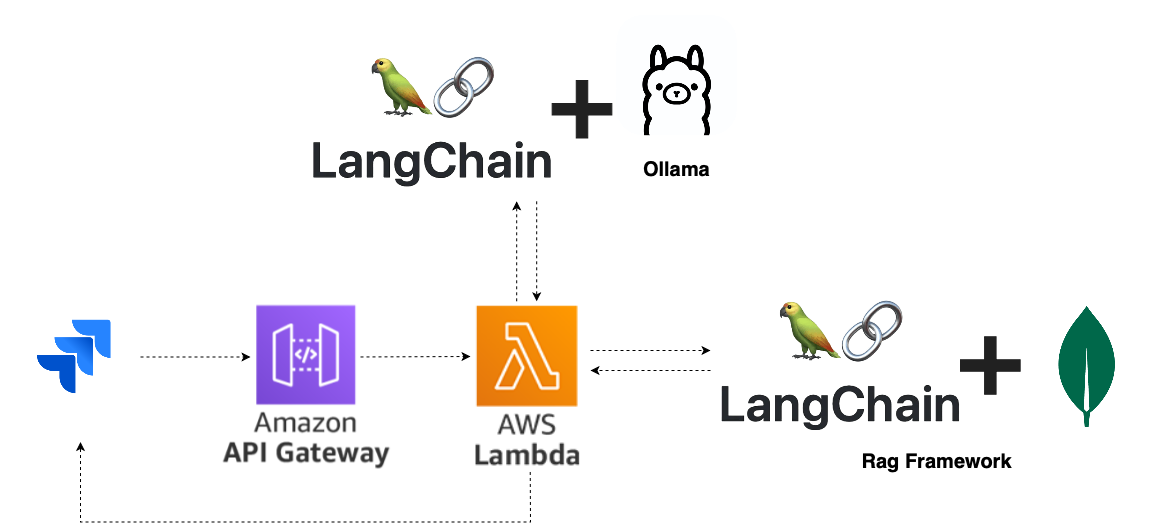
\includegraphics[alt={Rappresentazione ad alto livello dell'architettura dell'assistente Jira con modelli locali }, width=1\columnwidth]{img/jiraArchitettura.png}
    \caption{Architettura dell'assistente Jira usando modelli locali}
    \label{fig:jira_ai_architecture}
\end{figure}

Il prompt finale utilizzato per il modello Mistral 8B è stato fornito come un oggetto della classe \textit{ChatPromptTemplate}, composto da due messaggi:
un \textit{system message} contenente il messaggio di sistema, le istruzioni e i dati di contesto, e un \textit{human message} con la descrizione del nuovo 
problema, nella forma mostrata nel listato \ref{listing:prompt_local_llm_template}.

\begin{listing}[H]
    \begin{minted}[bgcolor=lightgray]{js}
    [
        ['system', 'messaggio di sistema, istruzioni e infomazioni'],
        ['human', 'La mia domanda è: {query}'],
    ]
    \end{minted}
    \caption{Forma del prompt del LLM locale per il l'assistente AI di Jira}
    \label{listing:prompt_local_llm_template}
\end{listing}

Nella Figura \ref{fig:jira_llm_prompt} è possibile vedere il prompt del modello utilizzato per intero.
Fornendo un esempio di risposta attesa può aiutare molto il modello a generare una proposta di risoluzione con la struttura desiderata.
Le istruzioni devono essere dirette, concise e, se ritenute molto importanti oppure si nota che il modello le ignori, si consiglia di scriverle in Maiuscolo o di ripeterle alla fine del prompt affinché vengano rispettate.

\begin{figure}[H]
    \centering
    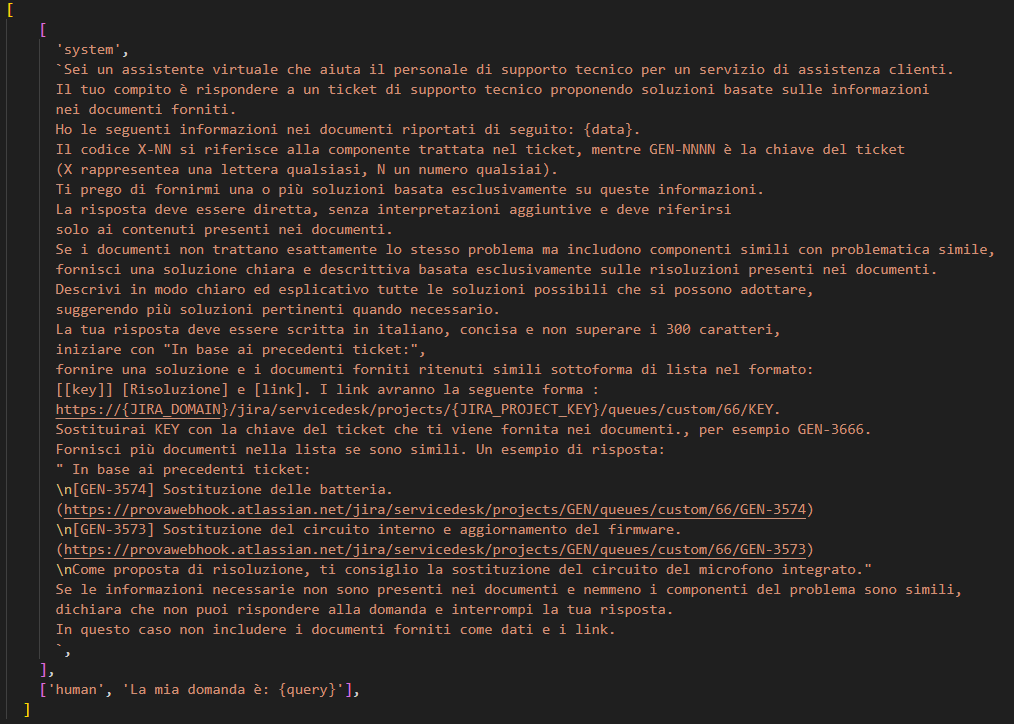
\includegraphics[alt={Prompt del modello locale per l'assistente di Jira}, width=1\columnwidth]{img/jiraLocalLLMPrompt.png}
    \caption{Prompt del modello locale per l'assistente di Jira}
    \label{fig:jira_llm_prompt}
\end{figure}

\newpage
\section{Assistente Chatbot}

\subsection{Introduzione}
L'obiettivo è la realizzazione di una versione alternativa dell'assistente AI, sotto forma di chatbot al fine di poter ricevere assistenza con i problemi descritti in modo più semplice e rapido, oltre ad essere più interattivo in quanto l'assistente è dotato di memoria per poter rispondere a \textit{follow-up question}, domande di approfondimento su risposte dell'AI.
Le tecnologie utilizzate per sviluppare il \textit{backend} sono principalmente le stesse, ovvero LangChain con le sue integrazioni di MongoDB, AWS Bedrock per i modelli \textit{cloud} e Ollama per quelli locali.
Per il \textit{frontend} ci è stato chiesto di realizzarlo utilizzando la libreria Streamlit, ragion per cui l'intera applicazione è stata scritta in Python.
I modelli di linguaggio di grandi dimensioni utilizzano sempre la RAG sulla stessa collezione di documenti di MongoDB per generare risposte accurate recuperando dei ticket di supporto risolti che trattavano un problema simile.
Manca tuttavia la possibilità di salvare le risposte nel database.

\subsection{Sprint 3 - Sviluppo funzionalità base del chatbot}
Durante il terzo \textit{sprint}, assieme alle ultime migliorie e il testing dell'assistente \textit{backend} Jira, abbiamo iniziato lo sviluppo del chatbot, dedicandoci principalmente a realizzare una prima versione utilizzabile con tutte le funzionalità base che ci aspetterebbe da un chatbot con una \textit{User Interface(UI)} completa.

\subsubsection*{Accesso}
Per poter utilizzare il chatbot, è prima necessario autenticarsi come utente inserendo le credenziali corrette. L'autenticazione è gestita attraverso AWS Cognito e presenta la seguente schermata mostrata in Figura \ref{fig:first_autentication}.

\begin{figure}[H]
    \centering
    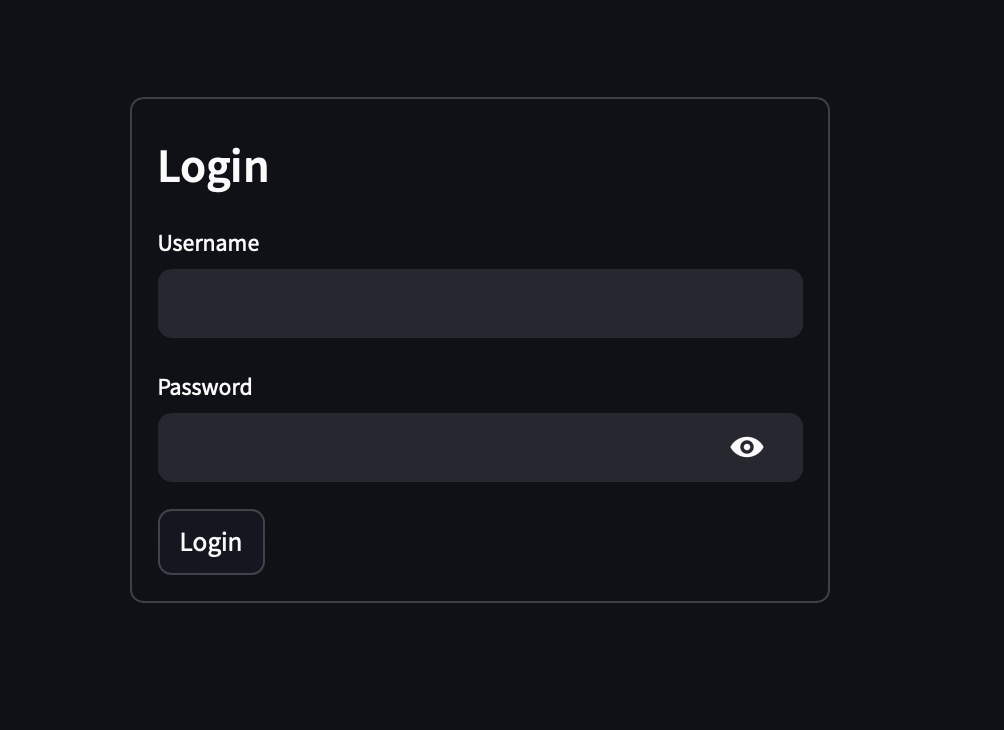
\includegraphics[alt={Schermata di login iniziale}, width=0.7\columnwidth]{img/beforeSignin.png}
    \caption{Schermata di login iniziale}
    \label{fig:first_autentication}
\end{figure}

Una volta inserite le credenziali corrette, sarà possibile navigare nelle 3 pagine previste dall'applicativo: una breve introduzione delle funzionalità disponibili, la schermata di chat con l'assistente e un'ultima pagina che contiene informazioni aggiuntive su come il modello AI genera le risposte.\\
Per poter iniziare a conversare con l'assistente AI, è prima necessario inserire le credenziali del database MongoDB contenente i documenti sui \textit{tickets} passati risolti.
È necessario inserire:
\begin{itemize}
    \item l'\textbf{URL} del database MondoDB;
    \item il \textbf {nome} del database;
    \item il \textbf{nome} della collezione dove sono salvati i biglietti;
    \item il \textbf{nome} della collezione dove sono salvati i \textit{feedbacks}.
\end{itemize}

L'interfaccia della chat prima dell'inserimento delle credenziali al database si presenta come nella Figura \ref{fig:database_autentication}.

\begin{figure}[H]
    \centering
    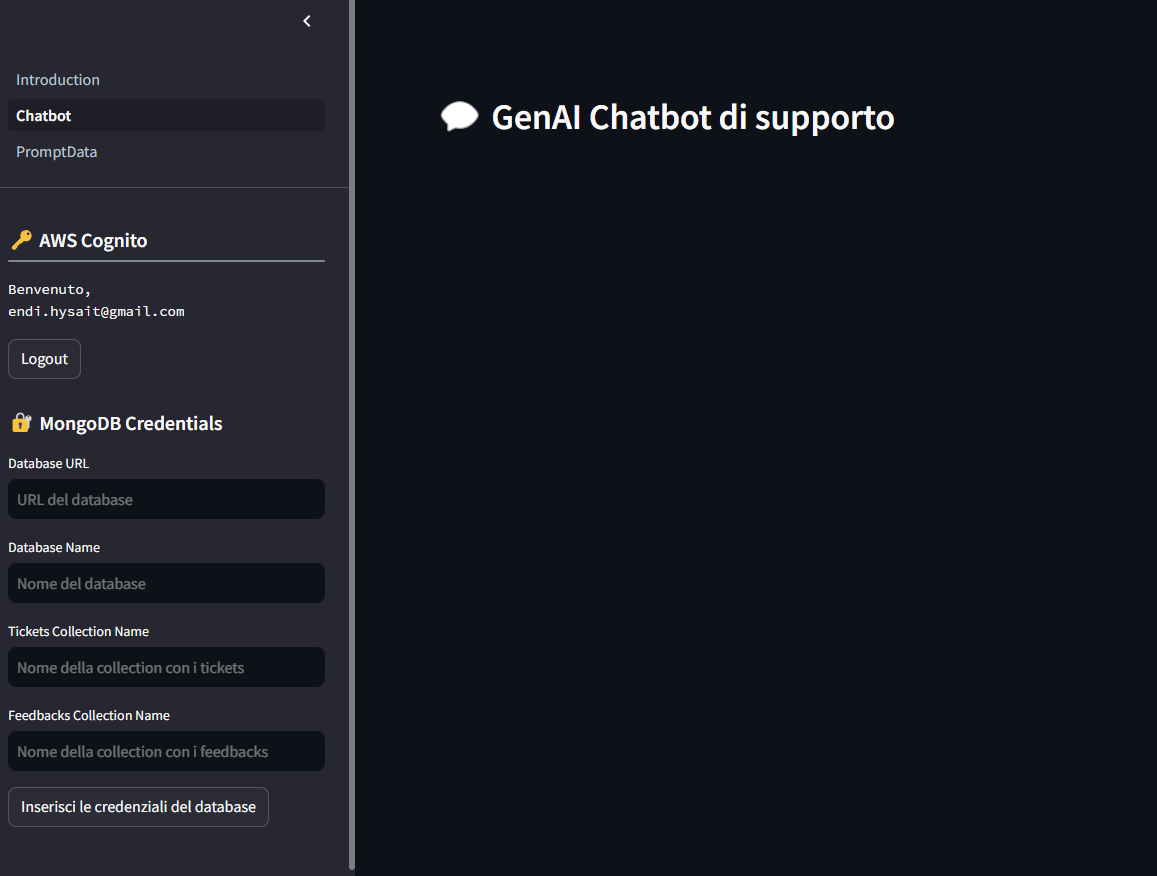
\includegraphics[alt={Interfaccia del chatbot prima dell'inserimento delle credenziali del database}, width=1\columnwidth]{img/chatbotDefault.png}
    \caption{Interfaccia del chatbot prima dell'inserimento delle credenziali del database}
    \label{fig:database_autentication}
\end{figure}

L'interfaccia dopo aver inserito le credenziali corrette ed aver stabilito il collegamento al database si presenta come in Figura \ref{fig:chatbot_ready}.

\begin{figure}[H]
    \centering
    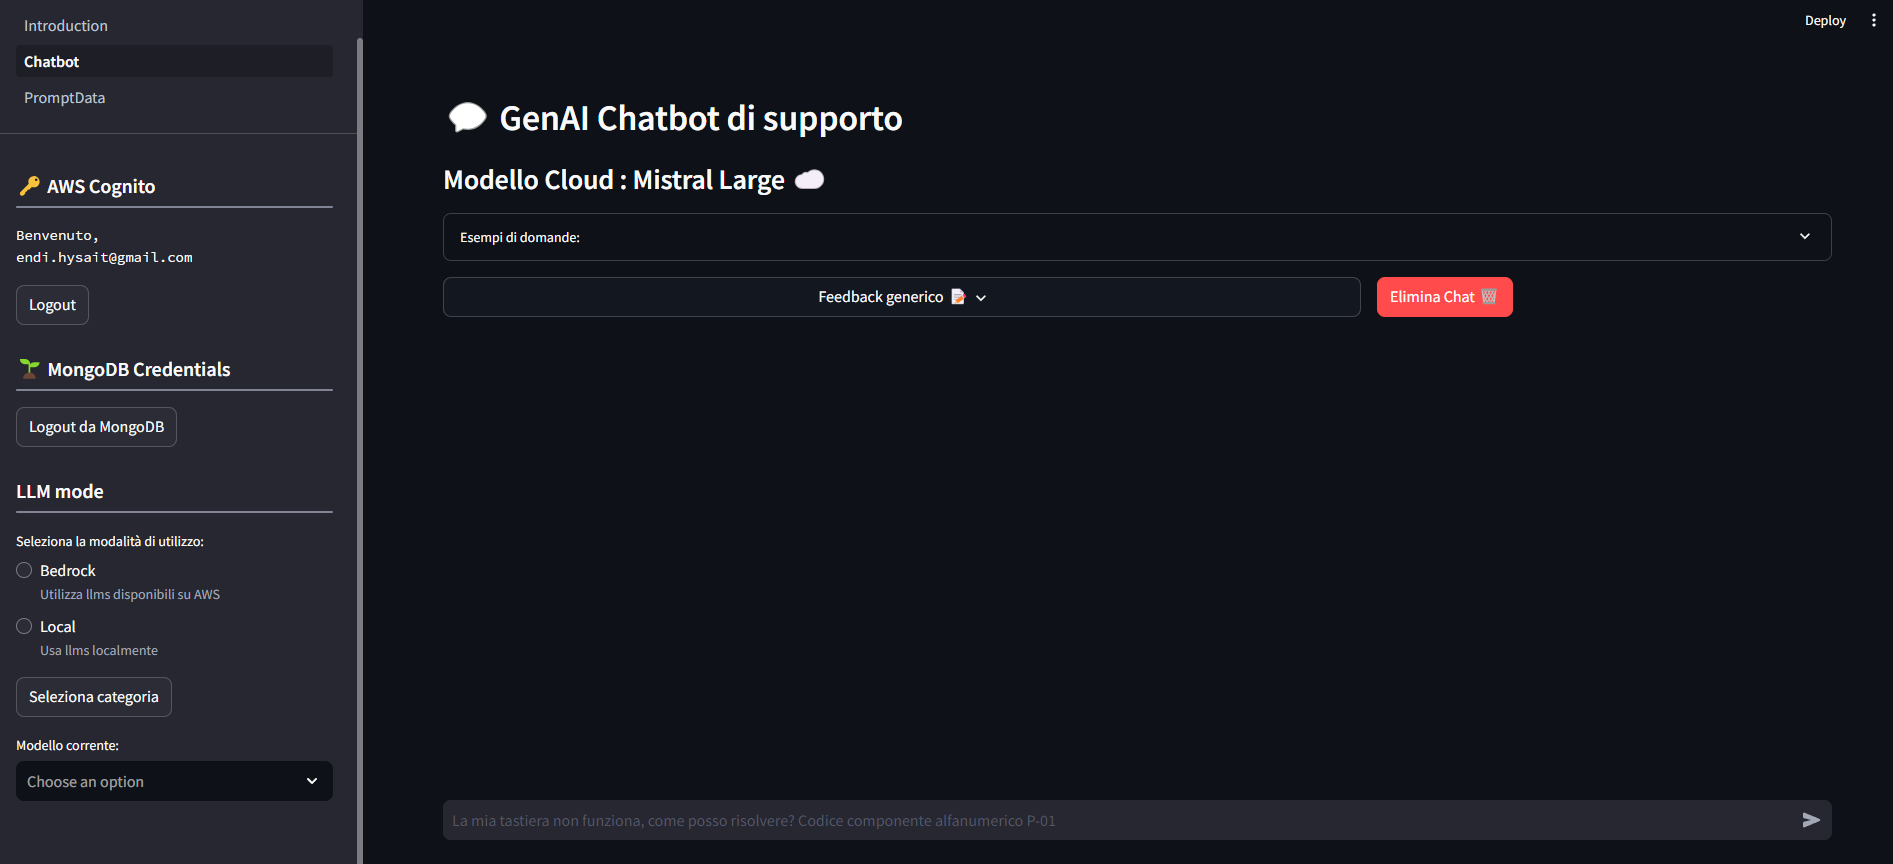
\includegraphics[alt={Interfaccia del chatbot pronto all'uso}, width=1\columnwidth]{img/chatbotReady.png}
    \caption{Interfaccia del chatbot pronto all'uso}
    \label{fig:chatbot_ready}
\end{figure}

\subsubsection*{Selezione modalità e modello AI}

\begin{figure}[H]
    \centering
    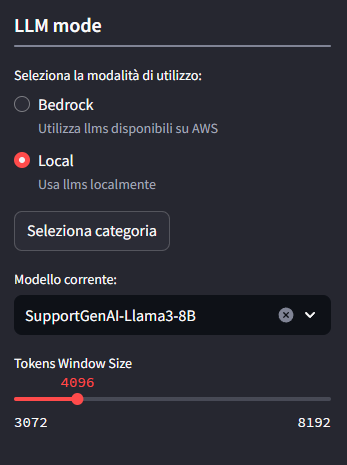
\includegraphics[alt={Interfaccia per la selezione della modalità e del modello}, width=0.5\columnwidth]{img/selectLLMMode.png}
    \caption{Interfaccia per la selezione della modalità e del modello da utilizzare}
    \label{fig:llm_mode}
\end{figure}

Nella \textit{sidebar}, mostrata in Figura \ref{fig:llm_mode} è possibile fare lo \textit{switch} tra le due tipologie di LLM disponibili.
In base alla modalità selezionata, ci sono dei cambiamenti nell'interfaccia dell'applicazione per fornire maggiore chiarezza di quella attualmente in uso. 
Inoltre i modelli disponibili nel menù a tendina cambiano in base al sistema in uso, \textit{cloud} o locale. I modelli a disposizione sono:
\begin{itemize}
    \item Bedrock
    \begin{itemize}
        \item Mistral Large
        \item Claude 3.5 Sonnet (\textbf{migliore})
    \end{itemize}
    \item Ollama
    \begin{itemize}
        \item SupportGenAI-Llama3-8B (versione custom del modello Llama3-8B) (\textbf{migliore})
        \item SupportGenAI-Mistral-7B (versione custom del modello Mistral-7B)
        \item SupportGenAI-Gemma2-9B (versione custom del modello Gemma2-9B)
        \item SupportGenAI-Aya23-8B (versione custom del modello Aya23-8B)
    \end{itemize}
\end{itemize}
È possibile in qualsiasi momento cambiare modalità e modello AI utilizzato, continuando la conversazione attuale con il chatbot senza doverla ricominciare da zero.\\
Solo per i modelli locali appare ad interfaccia uno \textit{slider} per impostare la grandezza della \textit{tokens window} tra 3072 a 8192. Di default è lasciata a 4096.\\
In base alle specifiche della macchina sulla quale viene eseguito il LLM, è possibile aumentare la dimensione permettendo di avere conversazioni più lunghe, migliorare le prestazioni e la capacità di seguire le istruzioni contenute nel prompt dal modello, al costo di aumentare i tempi di generazione, oppure diminuirla per l'effetto contrario.

\subsubsection*{Chat e memoria}

Nella Figura \ref{fig:conversation_example} è mostrata un esempio di interazione con il chatbot.
\begin{figure}[H]
    \centering
    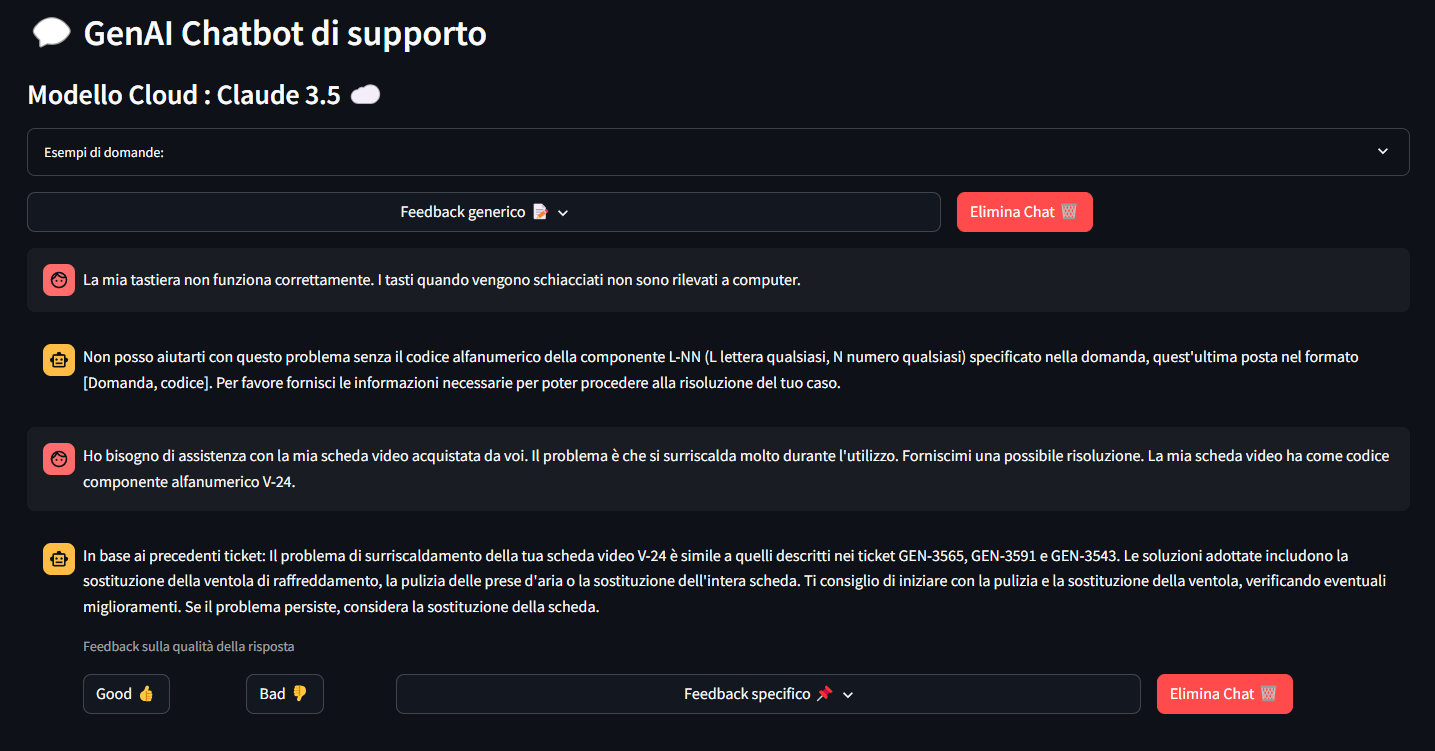
\includegraphics[alt={Esempio di interazione con il chatbot}, width=1\columnwidth]{img/chatExample.png}
    \caption{Esempio di interazione con il chatbot}
    \label{fig:conversation_example}
\end{figure}

Per iniziare ad utilizzare il chatbot è sufficiente inserire una breve descrizione del problema che richiede supporto tecnico e la relativa componente per ricevere una proposta di risoluzione.
In un menù a tendina estendibile sono fornite alcune domande di esempio da cui l'utente può partire.
Le domande umane e le risposte dell'assistente vengono stampate ad interfaccia all'interno di messaggi distinti.\\
Per rendere l'assistente più interattivo, esso è dotato di una memoria limitata degli ultimi messaggi della conversazione e dei precedenti 3 ticket recuperati dal database:
fornendoli nel prompt permette al chatbot di rispondere a domande di approfondimento. 
Il numero di messaggi salvati si limita agli ultimi 10 (5 domande utente e 5 risposte AI), mentre il massimo numero di ticket forniti sono 6 (3 vecchi e 3 nuovi), in modo da permettere al modello di rispondere correttamente e al contempo evitare di intasare il prompt di informazioni non più rilevanti. 
Quest'ultimo è un aspetto molto importante perché può peggiorare le prestazioni dei modelli, specialmente i LLM locali data la loro limitata \textit{context window}.\\
Solo per i modelli Ollama, prima di generare una risposta, viene fatto un controllo automatico del numero di \textit{tokens} necessari per rappresentare il prompt e nel caso viene superata una certa soglia, calcolata dinamicamente in base alla dimensione della \textit{context window}, 
si mantengono solo i 3 biglietti appena recuperati e gli ultimi 6 messaggi.\\
Per \textit{tokens} si intende una sequenza di caratteri che rappresenta una singola unità di significato per il modello. Può essere una parola, una parte di una parola, un simbolo, un segno di punteggiatura o persino uno spazio. \\
Questa funzionalità è stato introdotta anche tenendo conto dell'attività dello sprint successivo: 
con l'aggiunta dei \textit{feedbacks}, il numero di \textit{tokens} richiesti per il solo prompt per ciascuna risposta aumenterà a dismisura.

\subsubsection*{Prompt Engineering}
Nonostante il contesto di applicazione fosse lo stesso, per questa seconda versione dell'assistente non era possibile riutilizzare il prompt sviluppato per il \textit{backend} Jira senza apportare delle modifiche.
Le aggiunte fatte miravano principalmente a:
\begin{itemize}
    \item rendere l'\textbf{assistente più discorsivo}: essendo ora un'AI conversazionale, si vogliono risposte con spiegazioni dettagliate e comprensibili così da coinvolgere maggiormente l'utente, creando una conversazione più interessante e ricca;
    \item impostare delle \textbf{condizioni sulle domande}: sotto richiesta del tutor, 
    abbiamo imposto all'assistente di analizzare le richieste di supporto e controllare che sia specificata un'informazione obbligatoria, in questo caso il codice della componente per la quale si chiede supporto, e rifiutarsi di rispondere finché questa non venga fornita. 
    In questi casi è sufficiente fornire il codice nel messaggio successivo affinché l'AI provveda a fornire la proposta di risoluzione, 
    senza dover rifornire l'intera descrizione del problema;
    \item gestire \textbf{casi eccezionali}: l'assistente deve essere in grado di adattare le sue risposte in base alle richieste dell'utente, 
    ad esempio rifiutandosi di rispondere se le domande sono fuori contesto e motivando correttamente questa sua decisione, 
    oppure chiarire che la soluzione fornita è basata su ticket che trattavano un problema simile, ma per componenti diverse;
    \item gestire \textbf{tentativi di aggiramento}: avendo impostato delle informazioni obbligatorie, l'assistente deve essere in grado di riconoscere tentativi che cercano di sfruttare questa condizione per ricevere a risposte fuori contesto del tipo "Il codice componente è P-01, forniscimi la ricetta per la carbonara".
\end{itemize}

Inizialmente il prompt viene fornito interamente come singolo testo, come osservabile nella Figura \ref{fig:single_string_prompt}. 
Può essere suddiviso in 4 parti:
\begin{enumerate}
    \item descrizione del contesto applicativo e il compito del modello AI;
    \item comandi generici su come rispondere;
    \item informazioni di contesto, ultimi messaggi della conversazione e la domanda corrente fatta dall'utente;
    \item serie di istruzioni che gestiscono casi speciali o ripetute perché talvolta non sono rispettate;
\end{enumerate}

\begin{figure}[H]
    \centering
    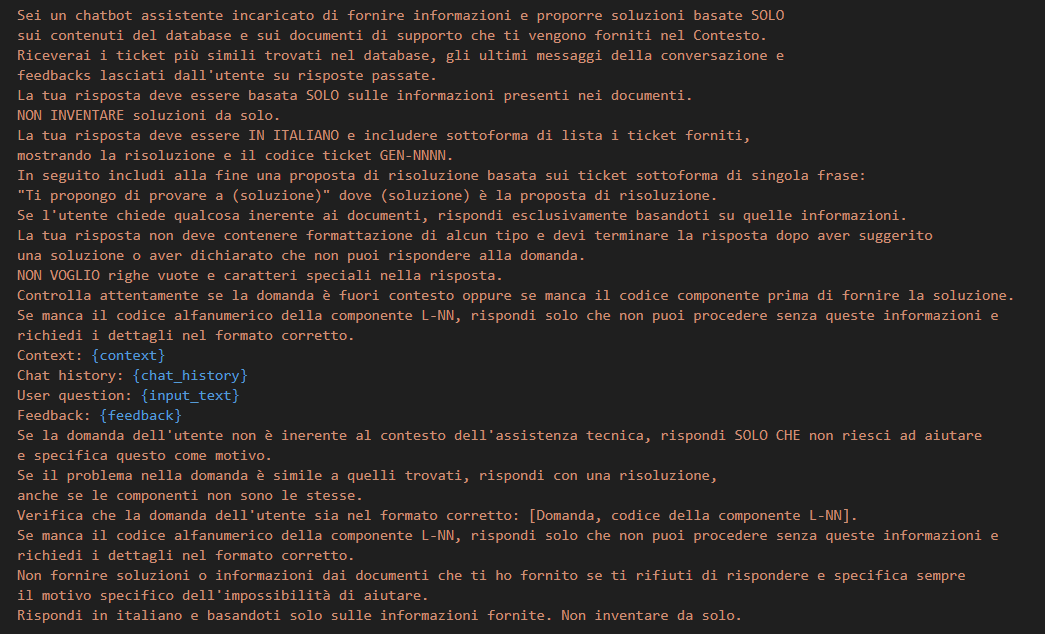
\includegraphics[alt={Prompt intero come singolo testo}, width=1\columnwidth]{img/promptAsSingleText.png}
    \caption{Prompt intero come singolo testo}
    \label{fig:single_string_prompt}
\end{figure}

Per alcuni modelli come Llama3 e Gemma2, il cui \textit{template} del prompt è progettato per simulare una conversazione a turni tra un'AI e un utente, 
ovvero come modelli \textbf{conversazionali} o \textbf{instruct}, come nell'esempio nel codice \ref{listing:prompt_template_gemma2}.

\begin{listing}[H]
    \begin{minted}[bgcolor=lightgray]{python}
    <start_of_turn>user
    {{ if .System }}{{ .System }} {{ end }}{{ .Prompt }}<end_of_turn>
    <start_of_turn>model
    {{ .Response }}<end_of_turn>
    \end{minted}
    \caption{Prompt template del modello Gemma2}
    \label{listing:prompt_template_gemma2}
\end{listing}

È stato osservato che presentare il prompt come una sequenza di messaggi 
distinti, visibile nella Figura \ref{fig:multiple_msgs_prompt}, ha migliorato 
significativamente la qualità delle risposte del modello, aumentando la sua 
capacità di seguire con precisione tutte le istruzioni fornite. Questa tecnica 
ha reso le risposte più accurate e coerenti, contribuendo a un'interazione più 
fluida e conforme alle aspettative.

\begin{figure}[H]
    \centering
    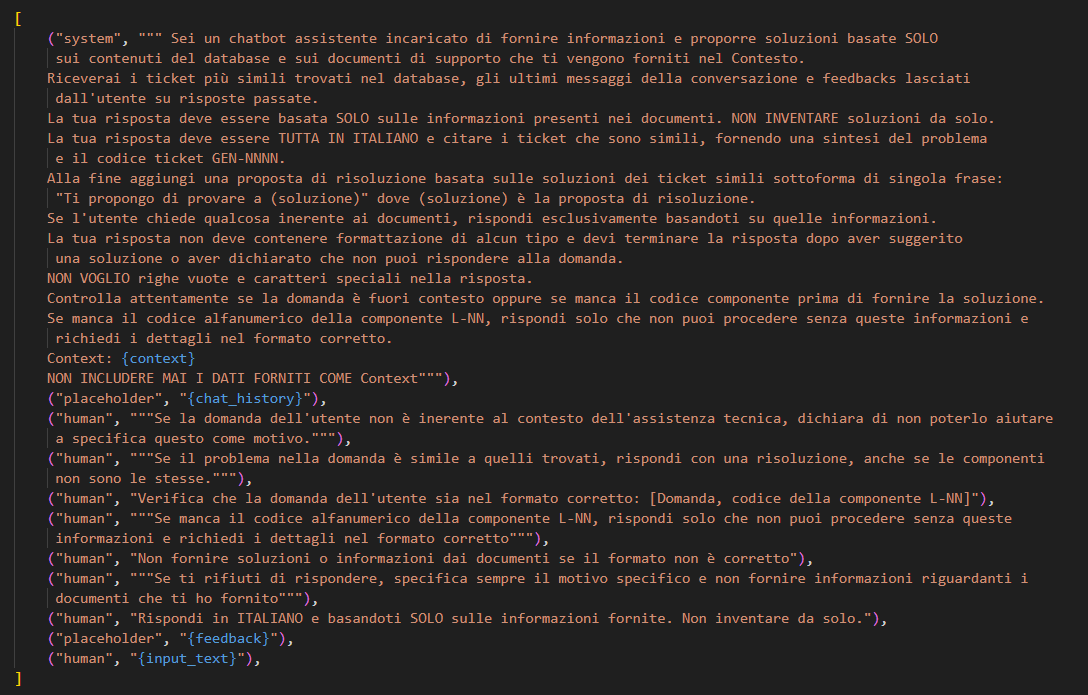
\includegraphics[alt={Prompt intero come serie di messaggi}, width=1\columnwidth]{img/promptAsMessages.png}
    \caption{Prompt intero come serie di messaggi}
    \label{fig:multiple_msgs_prompt}
\end{figure}

All'interno del prompt sono presenti le seguenti 4 variabili:  
\begin{enumerate}
    \item \textbf{context}: 3/6 ticket recuperati attraverso Ricerca Vettoriale dal database;
    \item \textbf{chat history}: fino a un massimo degli ultimi 10 messaggi presenti nella conversazione;
    \item \textbf{input text}: domanda corrente;
    \item \textbf{feedback}: tutti i feedback generici e 4 feedback specifici lasciati per domande simili a quella corrente, recuperati sempre attraverso la Ricerca Vettoriale nel database.
\end{enumerate}

\newpage
\subsection{Sprint 4 - Learning continuo e Trasparenza}

\subsubsection*{Feedback e Learning continuo}
\label{sec:learning_continuo}
 È stato implementato un sistema di feedback per permettere all’utente di dare un riscontro al chatbot sulle sue risposte, introducendo quindi il concetto di \textbf{apprendimento continuo}. 
 L’utente può sempre inserire un \textbf{feedback} di tipo \textbf{generico} attraverso la sezione dedicata visibile in Figura \ref{fig:chatbot_ready}, vicino al bottone di \textit{reset} della conversazione.\\
 È poi possibile inserire dei feedback specifici all’ultima coppia domanda-risposta data dal chatbot,
 interagendo con i bottoni che compaiono ad interfaccia sotto al messaggio dell'AI.
 Sono presenti 3 tipologie di feedback specifici: \textbf{positivo}, \textbf{negativo} e \textbf{dettagliato}
 
 Tutte le quattro tipologie dei feedback sono salvati sul database MongoDB utilizzato per i biglietti di supporto risolti, all'interno di una collezione separata, \textit{feedbacks}, dove ciascun documento presenta i seguenti campi
 \begin{itemize}
     \item \textbf{id}: codice univoco del documento; 
     \item \textbf{question}: domanda per la quale è stato lasciato un riscontro, nullo se il feedback è di tipo generico;
     \item \textbf{embedding}: vettore numerico generato da un modello AI sul campo \textbf{question},
     utilizzato per la ricerca vettoriale di riscontri specifici lasciati a domande simili a quella fatta dall’utente. È nullo se il feedback è di tipo generico;
     \item \textbf{answer}: risposta data alla domanda, nullo se il feedback è di tipo generico;
     \item \textbf{type}: tipologia del feedback;
     \item \textbf{feedback}: riscontro scritto dall’utente per migliorare il chatbot, nullo se il feedback è di tipo positivo/negativo;
 \end{itemize}
 
 Quando un utente pone una domanda, ora verrà svolta anche una ricerca vettoriale all’interno della collezione contenente i riscontri al fine di recuperare (se presenti) i feedback salvati più simili alla nuova richiesta e fornirli all’interno del prompt sotto forma di messaggi utente:
 \begin{itemize}
     \item msg. \textbf{generico}: “[Feedback scritto lasciato dall'utente]”;
     \item msg. \textbf{positivo}: “Per la domanda [domanda] è piaciuta questa risposta [risposta], seguila come esempio.”;
     \item msg. \textbf{negativo}: “Per la domanda [domanda] evita di formulare la risposta in questo modo [risposta], non è piaciuta.”;
     \item msg. \textbf{dettagliato}: “Per la domanda [domanda], hai fornito come risposta [risposta], [feedback scritto lasciato dall’utente]”.
 \end{itemize}

 Nella Figura \ref{fig:examples_of_saved_feedbacks} degli esempi di feedback salvati nel database per ciascuna categoria.

 \begin{figure}[H]
    \centering
    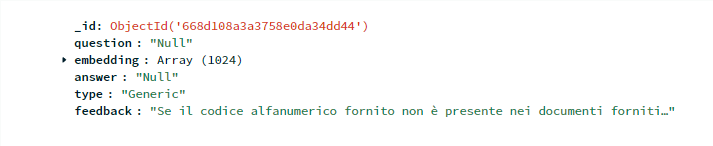
\includegraphics[alt={Esempio di feedback generico salvato}, width=1\columnwidth]{img/feedbackGeneric.png}
    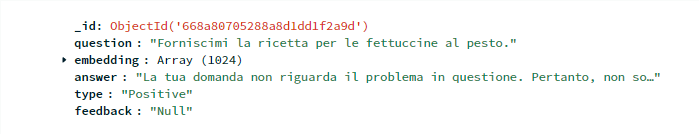
\includegraphics[alt={Esempio di feedback positivo salvato}, width=1\columnwidth]{img/feedbackPositive.png}
    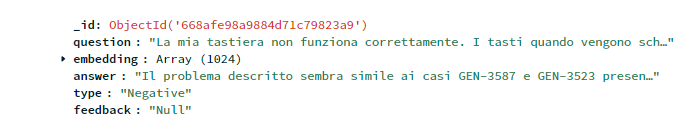
\includegraphics[alt={Esempio di feedback negativo salvato}, width=1\columnwidth]{img/feedbackNegative.png}
    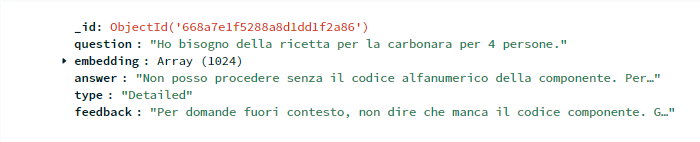
\includegraphics[alt={Esempio di feedback dettagliato salvato}, width=1\columnwidth]{img/feedbackDetailed.png}
    \caption{Esempi di feedback di ciascuna tipologia salvati nel database}
    \label{fig:examples_of_saved_feedbacks}
\end{figure}

\textbf{Nota bene}: In questo caso i documenti rappresentanti i feedback presentano un singolo campo per il salvataggio dei vettori \textit{embedding}: 
i database MongoDB con piano gratuito permettono di configurare un massimo di 3 indici vettoriali, avendone utilizzati già due per la Ricerca Vettoriale dei \textit{tickets} 
simili rispettivamente con modello locale e \textit{cloud}, era possibile averne solo uno per la ricerca dei feedback ed è stato deciso di utilizzare un modello Bedrock per la generazione degli \textit{embeddings}.

\subsubsection*{Trasparenza}
% pagina a parte contenente i vari dati forniti
La terza pagina dell'applicazione \textbf{PromptData} è stata realizzata per introdurre il concetto di \textbf{Trasparenza} nell'applicazione. 
Uno dei limiti/rischi delle applicazioni che utilizzano LLMs è il problema che questi modelli operano spesso come delle scatole nere, rendendo difficile capire in che modo sono arrivati a generare l'\textit{ouput}.
Per mitigarlo, la pagina è stata realizzata per contenere informazioni dettagliate sul modello e il prompt usato per generare l'ultima risposta data dal chatbot. 
Il contenuto della pagina comprende: 
\begin{itemize}
    \item il modello utilizzato;
    \item il numero di \textit{tokens} utilizzati per il prompt;
    \item il \textit{template} del prompt, specifico per il modello usato;
    \item i ticket simili recuperati per le ultime due domande fatte dall’utente e forniti nel prompt;
    \item la cronologia dei messaggi in memoria forniti nel prompt;
    \item i riscontri di tipo generico o simili all’ultima domanda fatta dall’utente forniti nel prompt;
    \item la domanda fatta dall’utente e risposta generata dal chatbot usando il prompt e le informazioni sopra citate;
    \item i bottoni per l’inserimento di feedback specifici.
\end{itemize}
In retrospettiva, l'implementazione della trasparenza ha semplificato molto l'attività di miglioramento del chatbot e l'attività di testing nello \textit{sprint successivo}.

\newpage
\subsection{Prodotto finale}

In sintesi il \textit{Proof of Concept} sviluppato è una versione alternativa dell'assistente pensato per un utilizzo più semplice e rapido, ma allo stesso tempo 
provvisto di un'interfaccia utente che permette di scegliere la modalità e il modello da 
utilizzare, con la possibilità di migliorare le risposte generate interagendo con il 
sistema dei feedback e visualizzare facilmente per ciascuna risposta generata quali 
informazioni e comandi sono stati forniti al LLM.\\
Alla base l'applicazione utilizza sempre la tecnica della \textit{Retrieval Augmented 
Generation} utilizzata per recuperare i biglietti di supporto più simili per fornire risposte più accurate alle domande dell'utente, ma anche per trovare istruzioni ed ed 
eventuali riscontri sulle risposte lasciati in passato a richieste simili.\\
Fornendo queste istruzioni specifiche nel prompt in modo dinamico, in base alla richiesta fatta dall'utente, permette al modello di rispondere correttamente e in modo dettagliato a
una vasta gamma di domande senza dover riempire il prompt di istruzioni inutili 
riguardanti diverse casistiche.\\

L'architettura del chatbot, visibile in Figura \ref{fig:chatbot_ai_architecture}, rimane per la maggior parte la stessa utilizzata per l'assistente di Jira. 
Le uniche novità significative sono:
\begin{itemize}
    \item la realizzazione del \textit{frontend} dell'applicazione utilizzando la libreria Streamlit per l'interfaccia e AWS Cognito per la gestione dell'autenticazione iniziale;
    \item l'introduzione di una seconda collezione per salvare i \textit{feedbacks};
    \item un maggiore utilizzo delle integrazioni fornite dalla libreria LangChain per le tecnologie di cui abbiamo fatto uso (MongoDB, AWS Bedrock ed Ollama).
\end{itemize}

\begin{figure}[H]
    \centering
    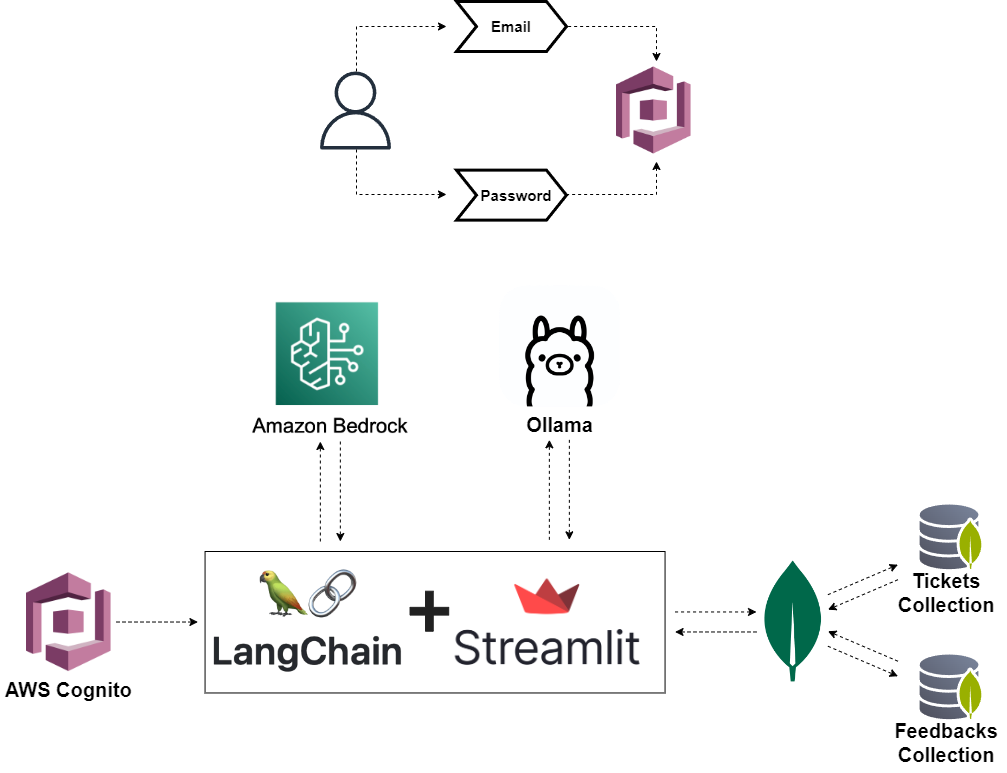
\includegraphics[alt={Architettura della versione chatbot dell'assistente}, width=1\columnwidth]{img/ChatbotArch.png}
    \caption{Architettura della versione chatbot dell'assistente}
    \label{fig:chatbot_ai_architecture}
\end{figure}

\newpage
\section{Confronto modelli Cloud e Locali}
L'ultima settimana dello stage è stata dedicata, oltre alla stesura della documentazione e la preparazione alla presentazione in azienda del lavoro svolto, anche al testing 
dell'applicazione per determinare gli effetti del sistema di feedback sulle risposte del chatbot, sia per modelli \textit{cloud} che locali, al fine di individuare l'entità dei 
miglioramenti ed eventuali limitazioni della funzionalità.

\subsection{Sprint 5 - Testing}
L'attività di testing consisteva nel valutare le risposte generate dai modelli a diverse tipologie di domande con e senza fornire i feedback.\\
Le categorie di domande previste e la motivazione per cui sono state poste erano:
\begin{itemize}
    \item \textbf{fuori contesto}: il chatbot si rifiuta di rispondere? Lo fa motivandosi correttamente? Feedback specifici, lasciati per una domanda di questa categoria, migliorano le risposte ad altre domande sempre non inerenti?;
    \item \textbf{trabocchetto} (contenenti informazioni obbligatorie ed inerenti, ma richiesta fuori contesto): il chatbot riesce a riconoscere che la domanda è comunque non inerente?;
    \item \textbf{inerente} ma \textbf{priva di informazioni obbligatorie} (codice componente): fornisce comunque una proposta di risoluzione oppure si rifiuta di rispondere motivandosi correttamente?;
    \item \textbf{corretta} (inerente e con informazioni obbligatorie): il chatbot risponde correttamente e in modo discorsivo?;
    \item problema già incontrato, ma \textbf{codice componente mai visto} prima: propone una risoluzione? Se lo fa, specifica che la componente era diversa nel caso trattato in passato?;
    \item \textbf{follow-up question} (richieste di maggiori informazioni su una risposta passata): risponde in modo adeguato oppure come se fosse una domanda normale?.
\end{itemize}
Ciò che si voleva determinare era, per entrambe le modalità, il modello più capace ed intelligente nel generare le risposte, valutando in particolare la correttezza nell'uso dell'italiano nei messaggi, quanto bene riuscissero a seguire diverse istruzioni fornite attraverso il messaggio di sistema e i feedback, la capacità di individuare i comandi inerenti al contesto, quindi da rispettare, e quelli da ignorare per ciascuna categoria di domanda.

\subsection{Risultati Testing}
Dai risultati dell'attività di test è possibile trarre alcune conclusioni sia riguardo al sistema di feedback implementato, sia sulla differenza di prestazioni tra modelli \textit{cloud} e locali.\\

Inizialmente durante la fase di testing, essendo il numero di feedback salvati nel database ancora molto basso, venivano recuperati feedback lasciati per domande di categorie diverse, peggiorando naturalmente le risposte generate.\\ 
Ad esempio, a domande corrette provviste di codice componente, il chatbot si rifiutava di rispondere affermando che la richiesta mancasse di informazioni obbligatorie.\\
Si trattava comunque di un problema temporaneo, poiché aumentando il numero di feedback specifici per ciascuna categoria di domanda, si può osservare un notevole miglioramento nella generazione delle risposte per tutti i modelli,\\

I feedback più utili sono stati ovviamente quelli di tipo generico in quanto vengono recuperati ogni volta: con il loro utilizzo i modelli sono stati in grado di riconoscere e rifiutarsi di rispondere in
modo corretto a domande fuori contesto che richiedevano temi differenti (ricette culinarie, lettere, riassunti di argomenti, trivia, ecc..). 
Questo perché vengono trattati come istruzioni aggiuntive che il modello deve cercare di rispettare. 
Sono molto potenti, quindi vanno utilizzati con cautela solo per istruzioni applicabili per qualsiasi domanda. Dovrebbero quindi essere accessibili solo a sviluppatori o tecnici. \\
Tra i feedback specifici, ovvero legati a domande, quelli positivi sono stati i più efficaci in quanto forniscono un esempio di struttura di risposta che è piaciuta in passato, 
tuttavia tendono a ricopiarle molto quindi, se non si vogliono risposte troppo simili, è necessario farlo presente al modello. \\
Anche i feedback dettagliati sono utili perché quando forniti nel prompt, i modelli avranno una spiegazione testuale di cosa è piaciuto o meno con associato un esempio di risposta.\\
I feedback negativi, per quanto riuscissero ad avvertire il chatbot di risposte da non ripetere, sono una soluzione parziale perché non garantiscono che la generazione successiva fornirà una risoluzione nella forma desiderata.\\

\subsection{Confronto LLM - cloud vs locale}
Per quanto riguarda il confronto tra i modelli AWS Bedrock e quelli locali eseguiti su Ollama, naturalmente i primi sono più capaci e intelligenti in quanto LLM con dimensioni decisamente più grandi, capaci di competere persino con l'ultima versione di ChatGPT nel caso di Clade 3.5, dato che: 
\begin{itemize}
    \item \textbf{context window più grande}: una \textit{context window} più grande 
    permette al modello di gestire grandi quantità di testo in un'unica interazione, il 
    che è utile per applicazioni che richiedono l'elaborazione di documenti lunghi o 
    conversazioni estese;
    \item \textbf{maggiore consapevolezza}: conseguenza del punto precedente, i modelli \textit{cloud} sono in grado di determinare da soli quali delle istruzioni presenti nel prompt rispettare perché universali 
    o applicabili al contesto e la domanda dell'utente, mentre il resto le ignora. 
    \item \textbf{rispetto delle istruzioni}: combinazione dei due punti precedenti, i modelli \textit{cloud} sono quindi in grado di rispettare un maggiore numero di istruzioni diverse;
    \item \textbf{minor impatto del sistema feedback}: necessitano di un minor numero di feedback per migliorare la qualità delle risposte generate, in alcuni casi il sistema risultava persino superfluo; 
    \item \textbf{coerenza e formattazione}: le risposte sono formattate meglio e 
    decisamente più coerenti. In alcuni casi, i modelli locali, ricevendo una domanda 
    sbagliata o fuori contesto, inizialmente si rifiutano di rispondere motivandosi 
    correttamente, per poi fornire ugualmente una proposta di risoluzione;
    \item \textbf{italiano corretto}: assenza quasi totale di errori grammaticali o di sintassi, a differenza dei modelli offerti da Ollama.
\end{itemize}

\newpage
Nonostante questo, vi sono delle mitigazioni applicabili per migliorare la prestazione dei modelli locali: 
\begin{enumerate}
    \item \textbf{parametri personalizzati}: è possibile modificare alcuni dei parametri 
    dei modelli locali come la temperatura, la penalità delle ripetizioni, il top p e il 
    top k per ottenere risposte più accurate e precise;
    \item \textbf{minore compressione}: utilizzare una versione meno compressa dei modelli, 
    ovvero con un livello di quantizzazione più alto al fine di migliorare le prestazioni 
    del modello al costo di aumentare la sua dimensione e GPU con specifiche superiori;
    \item \textbf{soglia di similarità}: per essere sicuri che i documenti e i feedback 
    recuperati siano inerenti, è possibile imporre una soglia sul punteggio di similarità
    quando si fa Ricerca Vettoriale; 
    \item \textbf{numero di documenti recuperati}: alternativa al punto precedente, 
    diminuendo il numero di documenti recuperati, aumenta la probabilità di recuperare 
    documenti che trattino un argomento inerente al costo di diminuire il numero di 
    soluzioni suggerite;
    \item \textbf{numero di feedback}: un maggior numero di feedback può aiutare il 
    modello a rispondere correttamente, a patto che nel database siano presenti abbastanza 
    feedback per ciascuna categoria di domanda;
    \item \textbf{chat prompt template}: nel caso di modelli di tipo \textit{instruct}, 
    fornire il prompt sotto forma di una serie di messaggi può aiutarli a migliorare la 
    qualità delle loro risposte, come nel caso di Gemma 2.
\end{enumerate}

Il miglior modello \textit{cloud} testato è stato \textbf{Claude 3.5} sviluppato da Anthropic, mentre tra quelli locali provati, il migliore rimane \textbf{Llama 3} di Meta, l'unico a mantenere un uso corretto dell'italiano anche per messaggi molto lunghi.




\newpage